\newpage
{\samepage
\begin{center}
{\Large{\bf Graphs}}
\end{center}
\begin{itemize}
\item A graph, $G$, consists of a set of vertices (nodes), $V$, together
with a set of edges (links), $E$, each of which connects two vertices.
\begin{center}
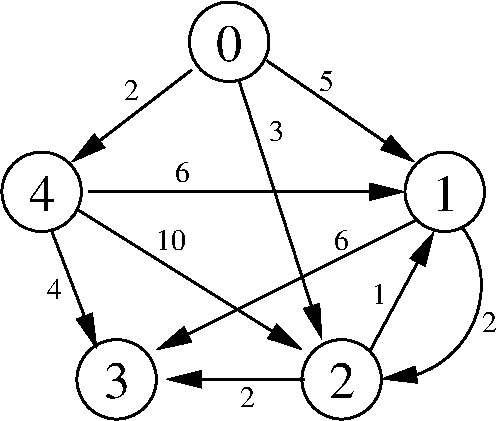
\includegraphics{../Images/grapha.pdf}
\end{center}
\item This is a directed graph (digraph).
Vertices are joined to adjacent vertices by these edges.
\item Every edge has a non-negative weight attached
which may correspond to time, distance, cost etc.
\end{itemize}
}

\newpage
{\samepage
\begin{center}
{\Large{\bf Graph ADT}}
\end{center}
{\small
\begin{verbatim}
#define INF (INT_MAX)

graph* graph_init(void);

int graph_addVert(graph* g, char* label);

bool graph_addEdge(graph* g,  int from,
                   int to, edge weight);

int graph_getVertNum(graph* g, char* label);

char* graph_getLabel(graph* g, int v);

edge graph_getEdgeWeight(graph* g, int from, int to);

int graph_numVerts(graph* b);

bool graph_free(graph* g);

/* Optional ? */
void graph_tostring(graph* g, char* str);

void graph_todot(graph* g, char* dotname);

/* Independant of Implementation type */
edge graph_dijkstra(graph* g, int from, int to);

edge graph_salesman(graph* g, int from, char* str);
\end{verbatim}
}}

\newpage
{\samepage
\begin{center}
{\Large{\bf Graph ADT II}}
\end{center}
The graph type could be implemented in a large number
of different ways.
\begin{itemize}
\item As two sets, one for vertices, one for edges.
We haven't looked at an implentation for sets, but one could use lists.
\item As an adjacency table - simply encode the weighted edges in a 2D array.
\begin{center}
\begin{tabular}{|c|ccccc|}\hline
& {\bf 0} & {\bf 1} & {\bf 2} & {\bf 3} & {\bf 4} \\ \hline
{\bf 0} & 0 & 5 & 3 & $\infty$ & 2 \\
{\bf 1} & $\infty$ & 0 & 2 & 6 & $\infty$ \\
{\bf 2} & $\infty$ & 1 & 0 & 2 & $\infty$ \\
{\bf 3} & $\infty$ &$\infty$ &$\infty$ & 0 & $\infty$ \\
{\bf 4} & $\infty$ & 6 & 10 & 4 & 0 \\ \hline
\end{tabular}
\end{center}
\end{itemize}
}

\newpage
{\samepage
\begin{center}
{\Large{\bf Realloc}}
\end{center}
{\small
\begin{verbatim}
graph* graph_init(void)
{
   int h, w;
   int i, j;
   graph* g = (graph*) ncalloc(sizeof(graph), 1);
   h = INITSIZE;
   w = h;
   g->capacity = h;
   g->adjMat = (edge**) n2dcalloc(h, w, sizeof(edge));
   g->labels = (char**) n2dcalloc(h,
                            MAXLABEL+1, sizeof(char));
   for(j=0; j<h; j++){
      for(i=0; i<w; i++){
         g->adjMat[j][i] = INF;
      }
   }
   return g;
}

edge graph_getEdgeWeight(graph* g, int from, int to)
{
   if((g==NULL) || (from >= g->size) ||
      (to >= g->size)){
      return INF;
   }
   return g->adjMat[from][to];
}

\end{verbatim}
}}

\newpage
{\samepage
\begin{center}
{\Large{\bf Realloc II}}
\end{center}
{\small
\begin{verbatim}
int graph_addVert(graph* g, char* label)
{

   int i, j;
   if(g==NULL){
      return NO_VERT;
   }
   if(graph_getVertNum(g, label) != NO_VERT){
      return NO_VERT;
   }
   /* Resize */
   if(g->size >= g->capacity){
      DO SOME RESIZING
   }
   strcpy(g->labels[g->size], label);
   g->size = g->size + 1;
   return g->size-1;
}

bool graph_addEdge(graph* g, int from, int to, edge w)
{
   if((g==NULL) || (g->size == 0)){
      return false;
   }
   if((from >= g->size) || (to >= g->size)){
      return false;
   }
   g->adjMat[from][to] = w;
   return true;
}
\end{verbatim}
}}

\newpage
{\samepage
\begin{center}
{\Large{\bf Linked}}
\end{center}
\begin{itemize}
\item As a Linked list:
\begin{center}
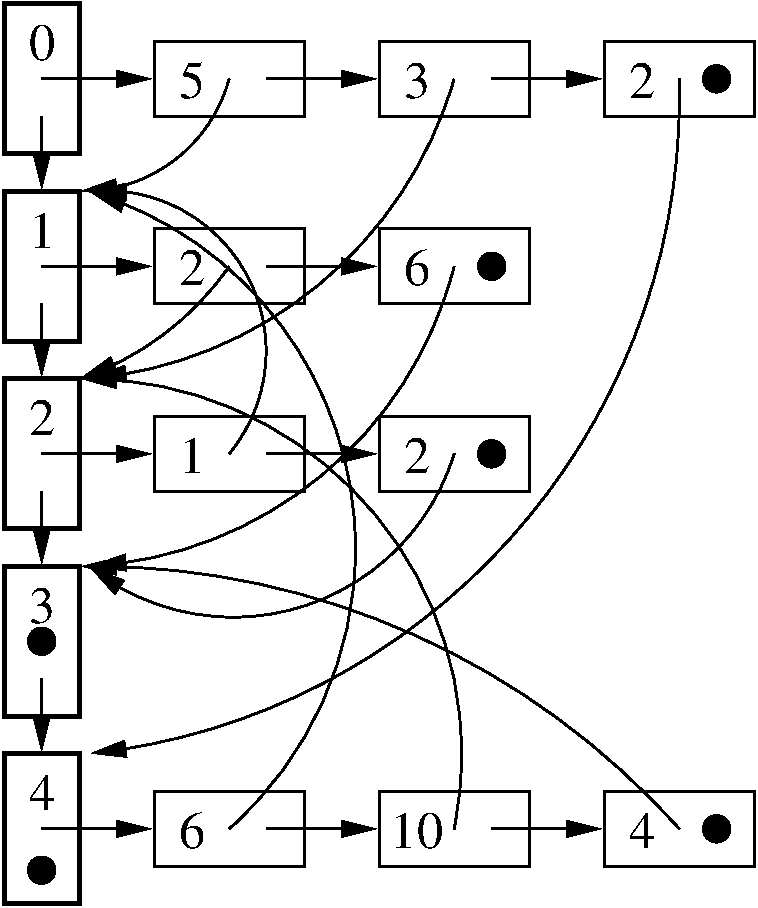
\includegraphics{../Images/graphll.pdf}
\end{center}
\end{itemize}
}

\newpage
{\samepage
\begin{center}
{\Large{\bf Linked II}}
\end{center}
{\small
\begin{verbatim}
graph* graph_init(void)
{
   graph* g = (graph*) ncalloc(sizeof(graph), 1);
   return g;
}

edge graph_getEdgeWeight(graph* g, int from, int to)
{
   int i;
   vertex *v;
   edgel* e;
   if((g==NULL) || (from >= g->size) ||
      (to >= g->size)){
      return INF;
   }
   v = g->firstv;
   for(i=0; i<from; i++){
      v = v->nextv;
   }
   if((v==NULL) || (v->num != from)){
      return INF;
   }
   e = v->firste;
   while(e != NULL){
      if(e->v->num == to){
         return e->weight;
      }
      e = e->nexte;
   }
   return INF;
}
\end{verbatim}
}}

\newpage
{\samepage
\begin{center}
{\Large{\bf Linked III}}
\end{center}
{\small
\begin{verbatim}
bool graph_addEdge(graph* g, int from, int to, edge w)
{
   vertex* f;
   vertex* t;
   int i;
   if((g==NULL) || (g->size == 0)){
      return false;
   }
   if((from >= g->size) || (to >= g->size)){
      return false;
   }
   f = g->firstv;
   for(i=0; i<from; i++){
      f = f->nextv;
   }
   t = g->firstv;
   for(i=0; i<to; i++){
      t = t->nextv;
   }
   return _addEdge(f, t, w);
}
\end{verbatim}
}}
